\documentclass[prl,twocolumn,superscriptaddress]{revtex4}
% \documentclass[twocolumn, a4j]{jarticle}
\renewcommand{\figurename}{Fig.}
\pagestyle{plain}
\usepackage[dvipdfmx]{graphicx,color}
\usepackage{amsmath,amssymb,braket,float,bm,color,comment,physics}
% \usepackage{mathabx}
\usepackage[hang,small]{caption}
\usepackage[subrefformat=parens]{subcaption}
\captionsetup{compatibility=false}
\begin{document}

\title{Transport Phenomena of Granular Materials in a Highly Filled Rotating Cylindrical System}
% 高充填回転円筒系における粒体の輸送現象
\author{S. Yoneta, S. Inagaki}
\affiliation{Dept. of Physics, Kyushu University}

\begin{abstract}
The advection structure is investigated by filling a concentric double cylinder with monodisperse particles and rotating it with the axis of the cylinder horizontal. In this experiment, we assumed passive scalar transport of a two-component system of white and colored particles, which differ only in color from white particles. The surface of the cylinder during the rotation and the cross section after the rotation were photographed to quantify the advection of colored particles. We propose an axial velocity distribution model that satisfies the characteristics of the advection structure (experimental facts). Using the conservation of flow rate derived from the assumption of incompressible material and the law of conservation of mass, we derive the relationship between the axial velocity in the surface layer and the inner layer, and the relationship between the axial velocity and the radial velocity in the inner layer. We formulate an advection equation in which the velocity field is spatially dependent, and obtain the existence ratio of colored particles by the finite difference method. Finally, the model is qualitatively evaluated by comparing the experimental observations with the numerical solutions obtained by simulation.
\end{abstract}
\maketitle

% \paragraph{I. INTRODUCTION:}
%%%%%%%%%%%%%%%%%%%%%%%%%%%%%%%%%%%%%%%%%%%%%%%%%%%%%%%%%%%%%%%%%%
%%%%%%%%%%%%%%%%%%%%%%%%%%%%%%%%%%%%%%%%%%%%%%%%%%%%%%%%%%%%%%%%%%
{\bf I. INTRODUCTION} \\
食品,医薬品,化学の製造プロセスにおいて混合を行うことがある.粉体の混合への理解は重要.\\

粉粒体には通常の流体や固体には見られない興味深い特性がある. その一つのとして, 二分散系回転円筒における分離現象がある. 粒径の異なる2種類の粒子を円筒内にいれ, 回転させると分離現象が起こり, 円筒の表面において中央から両端への移流が観察されている \cite{Inagaki15:bidisperse}. また, 部分充填二分散系において内部構造を探る試みは, MRI \cite{Hill97:MRI},  陽電子放出粒子追跡(PEPT) \cite{Ding01:PEPT}, 凝固剤による固化 \cite{Santomaso04:solid}などのさまざまな手法が使用されてきました.ただしこれらの手法は, 高額な実験装置が必要であったり, 実験に手間のかかります. また, 部分充填においては移流構造の研究が進んでいるが, 高充填は構造的に内部を観察することが困難です. \\
% 卓上塩を使った実験で内部がみえたのは意外だった. ガラスビーズで試してみた(黒色粒子はアルミナ1粒子)が, 下から照明を当てても見えなかった. 光が散乱して半透明になったのが原因かも?
% 参考文章(Santomaso04:solid)
\begin{comment}
In order to make a dynamical analysis of the interior of a granular bed, different techniques have been used such as the positron emission particle tracking (PEPT) (Bruno and Bridgwater, 2000; Ding et al., 2001; Parker et al., 1997) and the magnetic resonance imaging (MRI) (Nakagawa et al., 1993 or Hill et al., 1997; Ristow and Nakagawa, 1999). Such techniques, however are quite complex to set up and can be made only in specialized laboratory.
\end{comment}

今回我々は, サイズ分離現象で見られた移流が単分散系においても観察されるか調べるために, 高充填単分散系における内部構造の観察を行いました. 
二分散系の場合は,自発的にバンドが形成されるため,移流を定量化することは比較的容易である.しかし,単分散系においてはバンドが形成されないため,初期状態において円筒内の粒子の一部を着色し,着色パルスの時間発展の軌跡を観察することで,移流を可視化した.この手法によって, 高充填において円筒の表面だけでなく, 内部の軌跡を非侵襲で継続的に可視化することに成功した. \\
\\*
% 内部の移流の連続的な時間発展を可視化した先行研究はあるのか?
% 一部の粒子を着色することで, 移流を可視化する手法を用いた. 実験後は脱色することで, 再利用を可能にした. \\
%%%%%%%%%%%%%%%%%%%%%%%%%%%%%%%%%%%%%%%%%%%%%%%%%%%%%%%%%%%%%%%%%%
%%%%%%%%%%%%%%%%%%%%%%%%%%%%%%%%%%%%%%%%%%%%%%%%%%%%%%%%%%%%%%%%%%
% EXPERIMENT METHOD
The experiments were performed using monodisperse spheres in an acrylic transparent co-axial cylinder.
% with a hollow space between the outer and inner circles. 
The cylinder has inner $r_i$ and outer $r_s$ radii of 20 and 40 $\rm{mm}$, respectively, and a length $L$ of 345 $\rm{mm}$. 
For direct observation of the cross section, the drum was cut into two semi-cylinders and bolted together so that they could be separated after rotation.
%The general shape of the concentric double cylinder is the same as that of the study presented by Inagaki \it{et al.} \cite{Inagaki15:bidisperse}. 
We used spherical alumina beads 280±70 $\rm{\mu m}$ in diameter and 3.8 $\rm{g/cm^3}$ in density. %, white in color
To visualize the flow field inside the cylinder, we used particles of two different colors, white and red.
The alumina beads are originally white, and the red particles were colored with oil-based magic ink. (青い時もあるけど。)
We placed the cylinder vertically, and poured alternately white and colored particles into the cylinder to achieve a fill level of 95$\%$.
The fill level was defined as the volume of particle normalized by $64\%$ (random close packing) of cylinder volume. \\
By measuring the displacement of the pulses, the flow field can be measured.
Then, the cylinder was placed on two horizontal, parallel shafts. %horizontally
The cylinder was rotated at 15 $\rm{rpm}$ by driving one of the shafts by a brushless DC electric motor (Oriental Motors). Digital images of the entire cylinder were taken at constant intervals. 
We converted the images to grayscale, so colored particle is shown in black. We made a spatio-temporal diagram by the image sequences. The horizontal axis is the axial space on the surface and the vertical axis is time. It was created by vertically joining the axial vectors at each time.
The experimental method is essentially the same as that used by Inagaki \cite{Inagaki15:bidisperse}.

%%%%%%%%%%%%%%%%%%%%%%%%%%%%%%%%%%%%%%%%%%%%%%%%%%%%%%%%%%%%%%%%%%
%%%%%%%%%%%%%%%%%%%%%%%%%%%%%%%%%%%%%%%%%%%%%%%%%%%%%%%%%%%%%%%%%%
% EXPERIMENT RESULT
\begin{figure}[tb]
	\centering
	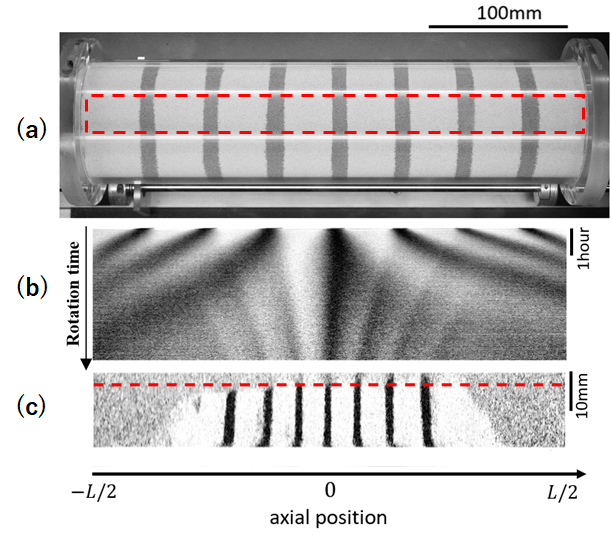
\includegraphics[width=0.5\textwidth]{figure/24_gray.png}
	\caption{実験1は充填率95%,回転時間が5時間である.(a-1) セットアップの画像.円筒を上から撮っている. (a-2) 時空間プロット. (a-3) 断面 見やすさのため断面のアスペクト比を変更している.}
	\label{fig:Expt.1}
\end{figure}

First,  inorder to observe the overall picture of the flow,
Expt.1 was performed with seven colored pulses placed at equal intervals in the initial state (Fig. \ref{fig:Expt.1}(a)). 
In Fig. \ref{fig:Expt.1}(b), the spatio-temporal diagram demonstrates the flow field at the surface of the cylinder. There are prominent trajectories of the seven pulses moving from the initial position to both end-walls. This indicates that flow from the center to the end-walls occurs on the surface of the cylinder.
It should be noted that there are also blurry trajectories from the initial positions of the pulses
to the center of the cylinder.
After a rotation of 5 hours, we opened the co-axial cylinder and observed the cross-sections.
Fig. \ref{fig:Expt.1}(c) is one of the cross-sections of the co-axial cylinder.
The upper and lower edges of the cross-section are the outer and inner cylinder.
The cross-section shows that the inside of the cylinder has two domains.
In the domain near the center of the inner cylinder, %the particles of two components (white and colored) are not mixed. T
the pulses move towards the center while remaining parallel.
There is a one-to-one correspondence between the position of the colored pulses of the cross-section and the final position of the blurry trajectories on the spatio-temporal diagram. The fact indicates that the blurry trajectories is the time evolution of the colored particles that spring from the unmixed domain to the surface. 
(再現性は確認してあります。)
%前回ここまで
% We performed several experiments by changing the fill level and the rotation speed of the cylinder, and the same results were confirmed \cite{supplement}. 
% (あとで直す)It would seem that the axial velocity in this domain is independent of the radial direction.
% In addition, we assume that the inside of the cylinder is composed of two layers. It is important to note that the two layers as a structure we have just assumed are different from the two domains (mixed and unmixed) described above. 

The trajectories of the colored pulses at both ends do not asymptote at the end-walls. This indicates that the velocity at the end-walls is not zero.

We assumed that the thickness of the surface layer is the same as that of the mixing domain near the center of the cylinder and is constant regardless of the axial position. We represent the layer boundary on the cross-section as a dashed line. We call the upper side surface layer and the lower side inner layer based on the layer boundary. Near the edge of the cylinder, the reason why the layer boundary doesn't coincide with the domain (mixed and unmixed) boundary is that the particles mixed in the surface layer sink into the inner near the edge.

In summary, in the inner layer, the blurry trajectories show particles move from both end-walls to the center. At the center, particles gush out the surface. In the surface layer, the prominent trajectories show particles move from the center to both end-walls. At both end-walls, particles sink into the inner layer. We assumed that the internal structure of the cylinder consists of two vortices, one clockwise in the right half and the other counterclockwise in the left half. The most remarkable fact to emerge from the data is that we can non-invasively observe the position of the pulses of the inner.

\begin{figure}[tb]
	\centering
	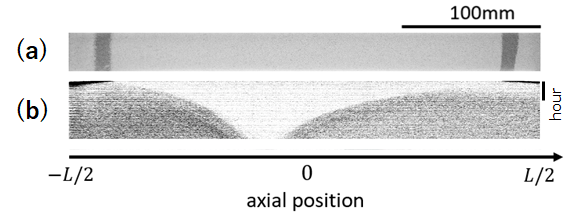
\includegraphics[width=0.5\textwidth]{figure/42_gray.png}
	\caption{実験2は充填率95%,回転時間が??時間である. (b-1) セットアップの解析領域の画像  (b-2) 時空間プロット.}
	\label{fig:Expt.2}
\end{figure}

Next, in order to quantify the axial velocity of the inner layer, Expt.2 was performed with two colored pulses, one at the left end-wall and the other at the right end-wall of the cylinder in the initial condition (Fig. \ref{fig:Expt.2}(a)). The spatio-temporal diagram shows the prominent trajectory toward the edge and the blurry trajectory toward the center. The inner edge of the blurry trajectories are the trajectories of the inner layer. The trajectories of the inner layers met after 〇 hours. This indicates that the velocity is not zero at the center of the advection structure.
\begin{figure}[tb]
	\centering
	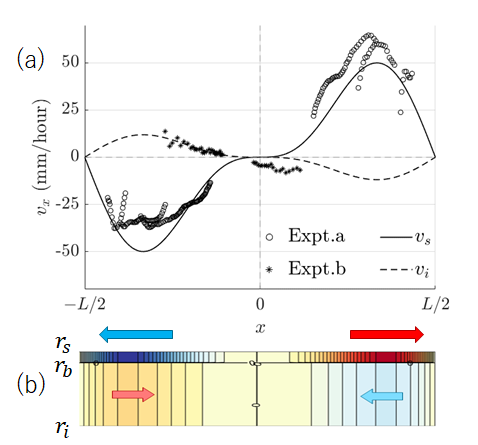
\includegraphics[width=0.5\textwidth]{figure/observed_and_model_vx.png}
	\caption{$v_x$の観測値とモデル.実験1から得られた表層軌跡の速度分布(o). 実験2から得られた内層軌跡の速度分布(*).}
	\label{fig:profile_model_vx}
\end{figure}
We calculated the velocities of the prominent trajectories (Fig.\ref{fig:Expt.1}(b)) and the blurry trajectories (Fig.\ref{fig:Expt.2}(b)), which are shown in Fig.\ref{fig:profile_model_vx}(a). $x$ is the axial coordinate with the center of the cylinder as the origin. We define axial velocities as $v_x$. \\
%%%%%%%%%%%%%%%%%%%%%%%%%%%%%%%%%%%%%%%%%%%%%%%%%%%%%%%%%%%%%%%%%%
%%%%%%%%%%%%%%%%%%%%%%%%%%%%%%%%%%%%%%%%%%%%%%%%%%%%%%%%%%%%%%%%%%
\\
{\bf I\hspace{-.1em}V. モデリング} \\
\qquad{\bf *. Overview of velocity distribution model(速度分布モデルの全体像)} \\
The reference of the axial position $(x=0)$ is the center of the cylinder. We consider a model in which the advection structure is symmetric in the $x=0$ plane. First, we explain the overall picture of the velocity distribution model, and later we explain the derivation of the velocity relation. We assume that $v_x\propto x^2\sin x$.  $v_x$ is $v_{smax}f_{norm}$ in the surface layer and $-v_{imax}f_{norm}$ in the inner layer (red line in Fig. \ref{fig:profile}). From the conservation of flow, $v_{imax}=v_{smax}({r_s}^2-{r_o}^2)/({r_o}^2-{r_i}^2)$ can be derived. The normalized $x^2\sin x$ function is $f_{norm}$ $(x'\equiv x/L, f\equiv {x'}^2\sin(2\pi x'),\hspace{5pt}f_{norm}\equiv f/max(f))$. When $r$ is constant, $v_r\propto dv_x/dx$ (blue line in Fig. \ref{fig:profile}). This is consistent with the experimental fact that the $x-v_r$ distribution model is bimodal. As shown in Fig. \ref{fig:overall}(d), the axial velocity field is smooth except for a discontinuity at the layer boundary $(r=r_o)$. The radial velocity field in the inner layer is smooth. \\
%%%%%%%%%%%%%%%%%%%%%%%%%%%%%%%%%%%%%%%%%%%%%%%%%%%%%%%%%%%%%%%%%%
\\
\qquad{\bf *. Governing equation(支配方程式)} \\
We define the densities, fluxes and velocities in the all-particles system as $\rho, \vb*{j}, \vb*{v}$, and in the colored particles system as $\rho_A, \vb*{j_A}, \vb*{v_A}$. From passive scalar transport, $\vb*{v} = \vb*{v_A}$. Fluxes are assumed to be advection-only, i.e. non-diffusive $(\vb*{j} = \rho\vb*{v},\hspace{5pt}\vb*{j_A} = \rho_A\vb*{v_A})$. By assuming incompressible matter, we can derive the incompressible flow from the law of conservation of mass in all-particles systems. From Gauss's divergence theorem, the flow rate is zero $\qty(\iint\nolimits_S\vb*{n}\vdot\vb*{v}dS = 0)$ at the surface $S$ in any volume region. This means that the inflow and outflow of particles passing over the surface $S$ are equal. From the assumptions of passive scalar transport, incompressibility, and axisymmetry and the conservation of mass in colored particles system $\qty(\partial\rho_A/\partial t+\div{\vb*{j_A}}=0)$, the advection equation 
\begin{equation} \label{eq:2Dae}
\pdv{\phi_A}{t}+v_r\pdv{\phi_A}{r}+v_x\pdv{\phi_A}{x} = 0
\end{equation}
can be derived. Note that the existence ratio $\phi_A(\equiv\rho_A/\rho)$ is the normalized $\rho_A$. From this, it can be seen that in order to solve the advection equation in colored particles system, we only need to design a velocity field model in all-particles systems. The $\phi_A$ is obtained by numerical calculation. \\
%%%%%%%%%%%%%%%%%%%%%%%%%%%%%%%%%%%%%%%%%%%%%%%%%%%%%%%%%%%%%%%%%%
\\
\qquad{\bf *. Derivation of 2D velocity field(2次元速度場の導出)} \\
From some assumptions and conservation laws, we derive the relation between the axial velocities of the surface layer and the inner layer, and the relation between the axial and radial velocities in the inner layer. First, the axial velocities in the surface layer and in the inner layer are denoted by $v_s, v_i$. The maximum axial velocities in the surface and in the inner layers are $v_{smax}, v_{imax}$, and we assume that $v_x$ is independent of $r$ in each layer $(v_x=v_x(x))$ and that the fill level is 100%. Since the flow rates passing left and right in any plane perpendicular to the rotation axis are equal $(\pi({r_o}^2-{r_i}^2)v_i+\pi({r_s}^2-{r_o}^2)v_s = 0)$, the velocity ratio between the surface and the inner layers \\
\begin{eqnarray} \label{eq:in_surf}
\dfrac{v_s(x)}{v_i(x)} = -\dfrac{{r_o}^2-{r_i}^2}{{r_s}^2-{r_o}^2}
\end{eqnarray}
is independent of $x$. Therefore, we can derive $v_i$ from $v_s$. \\

Next, we derive $v_r$ from $v_x$ in the inner layer. 
% The radial distance from the axis of the cylinder is defined as $r$. 
From the assumptions of incompressible flow, axisymmetry and no radial dependence of $v_x$ within each layer, it follows that \\
\begin{eqnarray}
v_r = -\dfrac{1}{2}\dfrac{dv_x}{dx}r+\dfrac{C(x)}{r}
\end{eqnarray}
$C(x)$ is an integration constant. We now consider the conservation law of the flow rate at the surface of the region $V$ in the inner layer. The range of the domain $V(r',\theta',x')$ is $r_i\leq r'\leq r(\leq r_o),\hspace{5pt}0\leq \theta'<2\pi,\hspace{5pt}x\leq x'\leq x+\Delta x$. Since the outflow in the axial direction is equal to the inflow in the dynamic direction, \\
\begin{eqnarray} \label{eq:vx_vr}
&& \pi\qty(r^2-{r_i}^2)\qty(v_x(x+\Delta x)-v_x(x))\nonumber \\
&=& \displaystyle\int_{x}^{x+\Delta x}dx\int_{0}^{2\pi}d\theta\hspace{2pt}(-v_r)r\nonumber \\
&\rightarrow& C(x) = \dfrac{{r_i}^2}{2}\dfrac{dv_x(x)}{dx}\nonumber \\
&\rightarrow& v_r(r,x) = -\dfrac{1}{2}\dfrac{dv_x(x)}{dx}\qty(r-\dfrac{{r_i}^2}{r})
\end{eqnarray}
Because of piston flow in the surface layer, the particles are homogenized in the radial direction. Therefore, $v_r$ is undefinable. \\

\begin{figure}[tb]
	\centering
	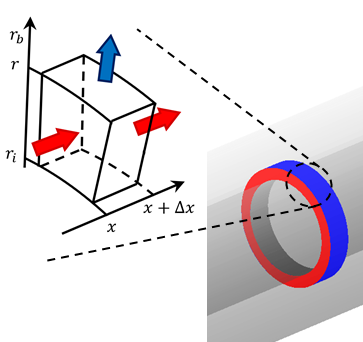
\includegraphics[width=0.5\textwidth]{figure/vx_vr_inner4.png}
	\caption{内層における軸方向速度と動径方向速度の関係の導出}
	\label{fig:vx_and_vr}
\end{figure}
\begin{figure}[tb]
	% \vskip10mm
	\centering
	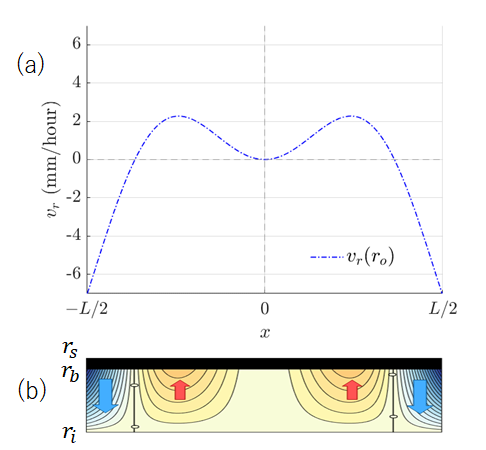
\includegraphics[width=0.5\textwidth]{figure/model_vr.png}
	\caption{$v_r$のモデル}
	\label{fig:model_vr}
\end{figure}

Therefore, the relation between the axial velocities in the surface layer and the inner layer Eq. \ref{eq:in_surf} and the relation between the axial velocity and the radial velocity in the inner layer Eq. \ref{eq:vx_vr} can be derived. From Eq. \ref{eq:vx_vr}, the flow function is $v_x(r^2-{r_i}^2)/2$. This satisfies the relation between the flow function and the velocity in the cylindrical coordinate system. Since the velocity field is stationary, the streamline and the trace line coincide. Therefore, the streamline in the inner layer (Fig. \ref{fig:streamline}) can be obtained analytically. Because of the piston flow in the surface layer, the trace line is meaningless. Therefore, the trace lines in the surface layer are omitted. \\
%%%%%%%%%%%%%%%%%%%%%%%%%%%%%%%%%%%%%%%%%%%%%%%%%%%%%%%%%%%%%%%%%%
%%%%%%%%%%%%%%%%%%%%%%%%%%%%%%%%%%%%%%%%%%%%%%%%%%%%%%%%%%%%%%%%%%
\\
{\bf V. SIMULATION DESCRIPTION} \\
% In this experiment, we assumed passive scalar transport in a two-component system, white and red particles. The passive scalar transport is that the existence ratio of the colored particles doesn't affect the velocity field, but follows the velocity field. 

The governing equation is the two-dimensional advection equation (Eq. \ref{eq:2Dae}), where $v_x$ and $v_r$ are substituted by the velocity field model described above. Using the finite difference method, we calculate $\phi_A$. For simplicity, we choose an explicit method in which the unsteady terms are forward differentials and the advection terms are first-order accurate upwind scheme. The staggered grid is chosen as the computation point and the Neumann condition is chosen as the boundary condition. In order to avoid divergence of the numerical solution, we set the tick size so that $\Delta t\qty(|v_r|/\Delta r+|v_x|/\Delta x)\leq1$ is satisfied. In order to avoid divergence of the numerical solution, we set the tick size so that $\Delta t\qty(|v_r|/\Delta r+|v_x|/\Delta x)\leq1$ is satisfied.  We set $\Delta r = \Delta x = 0.15$ (mm/cell)$ and \hspace{5pt}\Delta t = 4.5$ (sec/step). Because of the piston flow in the surface, $v_r$ is undefinable. However, the value of $v_r$ in the surface layer has to be set in order to perform the simulation. However, the value of $v_r$ for the surface layer has to be set in order to perform the simulation. Therefore, similarly to the relationship between $v_x$ and $v_r$ in the inner layer, we derive $v_r$ from the conservation of the flow rate at the surface of the region in the surface layer, and set this as the $v_r$ of the surface layer for the convenience on the simulation.  In order to reflect that the piston flow in the surface layer, $\phi_A$ is averaged in the radial direction after the finite difference calculation at each step. \\
%%%%%%%%%%%%%%%%%%%%%%%%%%%%%%%%%%%%%%%%%%%%%%%%%%%%%%%%%%%%%%%%%%
%%%%%%%%%%%%%%%%%%%%%%%%%%%%%%%%%%%%%%%%%%%%%%%%%%%%%%%%%%%%%%%%%%
\\
{\bf V\hspace{-.1em}I. SIMULATION RESULT} \\
\begin{figure}[t]
	\begin{minipage}[t]{0.95\linewidth}
		\centering
		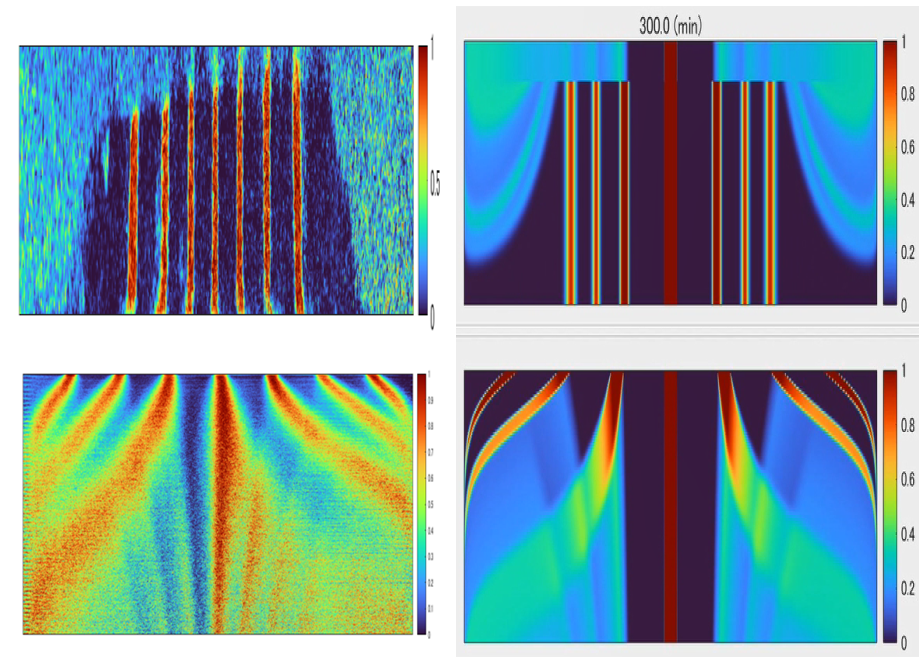
\includegraphics[width=\textwidth]{figure/24_exp_and_simu.png}
	\end{minipage}
	\begin{minipage}[t]{0.95\linewidth}
		\centering
		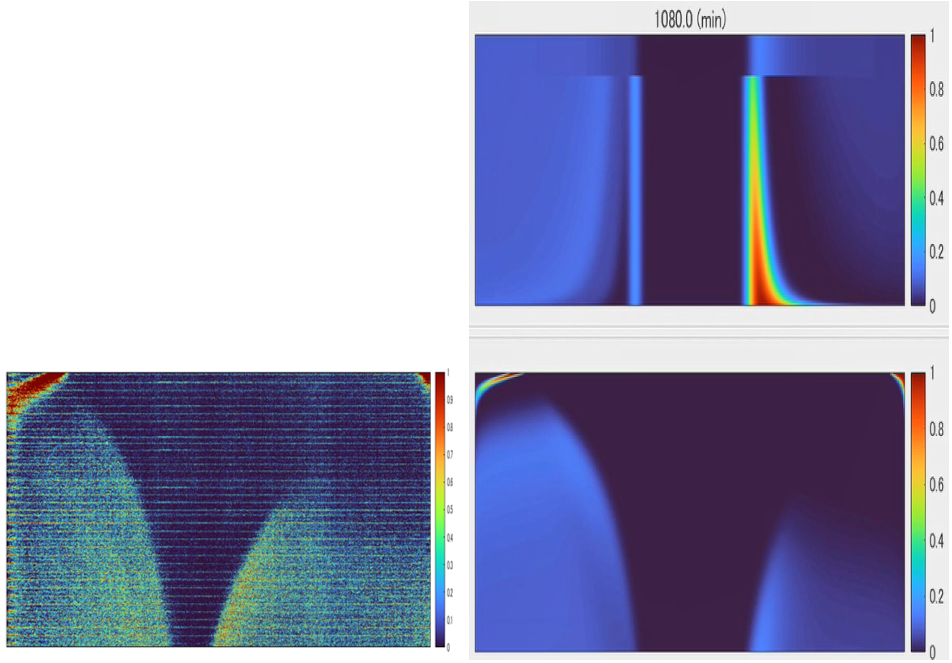
\includegraphics[width=\textwidth]{figure/38_exp_and_simu.png}
	\end{minipage}
	\caption{実験とモデルのシミュレーションの比較 (a)全体像 (b)両端}
	\label{fig:simu}
\end{figure}
The model was qualitatively evaluated by comparing the simulation results with the experiments. Fig. \ref{fig:simu}(a) shows the case where the seven colored pulses are evenly aligned in the initial state. First, we compared the experimental and model simulations in the cross section. In the experiment, it was observed that the mixture of white and colored particles arriving around the edge of the surface layer gradually spreads from the upper part of the edge of the inner layer toward the center, and the same feature appears in the model simulation. The model differs from the experiment in that no diffusion is observed in the center of the surface layer, because the governing equation of the model is the advection equation. Next, we compared the experimental and model simulations in the spatio-temporal diagram. Note that in the model, the advection structure is symmetrical, while in the experiment, the center of the structure is to the left of the center of the cylinder. It can be seen that the characteristics of the time evolution of the pulses at the center and around the edge are generally consistent between the experiment and the model. The model differs from the experiment in that the velocity of the pulse around the end-wall is asymptotically close to zero. \\
Fig. \ref{fig:simu}(b) shows the case where the initial state with one colored pulse around the left end-wall and one around the right end-wall. The observed fact that the trajectory of the inner layer does not appear in the initial stage, but only in the middle, is also shown in the simulation. \\
Fig. \ref{fig:simu}(c) shows the case where the colored particles are buried in the bottom of the inner layer in the initial state. \\
We have verified that the total mass of the colored particles is conserved in the simulation results, and found that the relative error per hour is less than 1% in most cases. Other tests to verify whether the model is solved accurately include comparing the velocity distribution of the model with that obtained from the simulation results, and comparing the trajectory of tracer particle (simulation) with the analytical solution of the streamlines obtained from the flow function (see supplement for details). \\
%%%%%%%%%%%%%%%%%%%%%%%%%%%%%%%%%%%%%%%%%%%%%%%%%%%%%%%%%%%%%%%%%%
%%%%%%%%%%%%%%%%%%%%%%%%%%%%%%%%%%%%%%%%%%%%%%%%%%%%%%%%%%%%%%%%%%
\\
{\bf V\hspace{-.1em}I\hspace{-.1em}I. CONCLUSIONS} \\
要約すると,実験から高充填二分散系の回転二重円筒内の粒子は渦型に移流することが確認できた.円筒中央において粒子が湧き出すことから,非侵襲的な表面観察だけで内層の速度分布を定量化することが可能になった.保存則に従い, かつ移流構造の特徴を捉えたモデルの提案を行った.二分散系において,サイズ分離により形成されたバンドが中央から両端に移流する現象が報告されているが,本研究により,二分散系由来のサイズ分離現象がなくとも,移流が起こることがわかった.
円筒を回転させると渦構造が形成される要因については,遠心力と壁面摩擦によるものであるという仮説を提案する.$r$が一定のとき,任意の軸方向位置において,遠心力は均一に働いているが,壁面は摩擦により相対的に中央よりも遠心力の影響が弱くなる.その結果,表層において中央で密に,両端で疎になる偏りが発生する.その偏りを緩和するために,表層においては中央から両端に粒子が流れると考える.同様の議論により,内層においては両端から中央に粒子が流れる.

今後の課題としては,3つのことを検討している.1つ目は,定量的なモデルの妥当性評価である.定性的には,モデルのシミュレーションは実験の特徴をよくとらえてるが定量的な評価はまだできていない.定量的にモデルの妥当性を評価するには,多くの実験データを必要とする.2つ目は,拡散を考慮したモデルの提案である.本モデルは移流方程式を支配方程式としており,拡散を考慮しないモデルとなっている.移流拡散方程式を支配方程式とする拡散を考慮したモデルを設計することにより,実験結果のより詳細な再現が可能になるかもしれない.シミュレーションにおいて拡散の発生が確認できるのは,速度場の空間依存性により,移流方程式が非線形になっているからである.例えば,Fig. \ref{fig:simu}(a-4)の左から3, 5番目のパルス拡散により幅が広がっている.3つ目は円筒の回転速度や充填率などのパラメータと速度場の関係の解明である.\\
\begin{eqnarray*}
\end{eqnarray*}

\begin{thebibliography}{}
\bibitem{Inagaki15:bidisperse}
S. Inagaki, H. Ebata and K.Yoshikawa, {\it{Phys. Rev. E}} {\bf 91}, 010201(R) (2015).
\bibitem{Hill97:MRI}
K. M. Hill, A. Caprihan, and J. Kakalios, {\it{Phys. Rev. Lett.}} {\bf 78}, 50 (1997).
\bibitem{Ding01:PEPT}
Y. L. Ding, J. P. K. Seville, R. Forster and D. J. Parker, {\it{Chem. Eng. Sci.}} {\bf 56}, 1769-1780 (2001).
\bibitem{Santomaso04:solid}
A. Santomaso, M. Olivi and P. Canu, {\it{Chem. Eng. Sci.}} {\bf 59}, 3269-3280 (2004).
\bibitem{supplement}
See Supplemental Material at .
\bibitem{LeVeque07:FDM}
R. J. LeVeque, {\it{Finite Difference Methods for Ordinary and Partial Differential Equations}} (University of Washington, Washington, 2007).
\bibitem{Batchelor00:fluid}
G. K. Batchelor, {\it{AN INTRODUCTION TO FLUID DYNAMICS}} (Cambridge University Press, Washington, 2000).
\end{thebibliography}

\end{document}